\begin{figure}[p]\centering
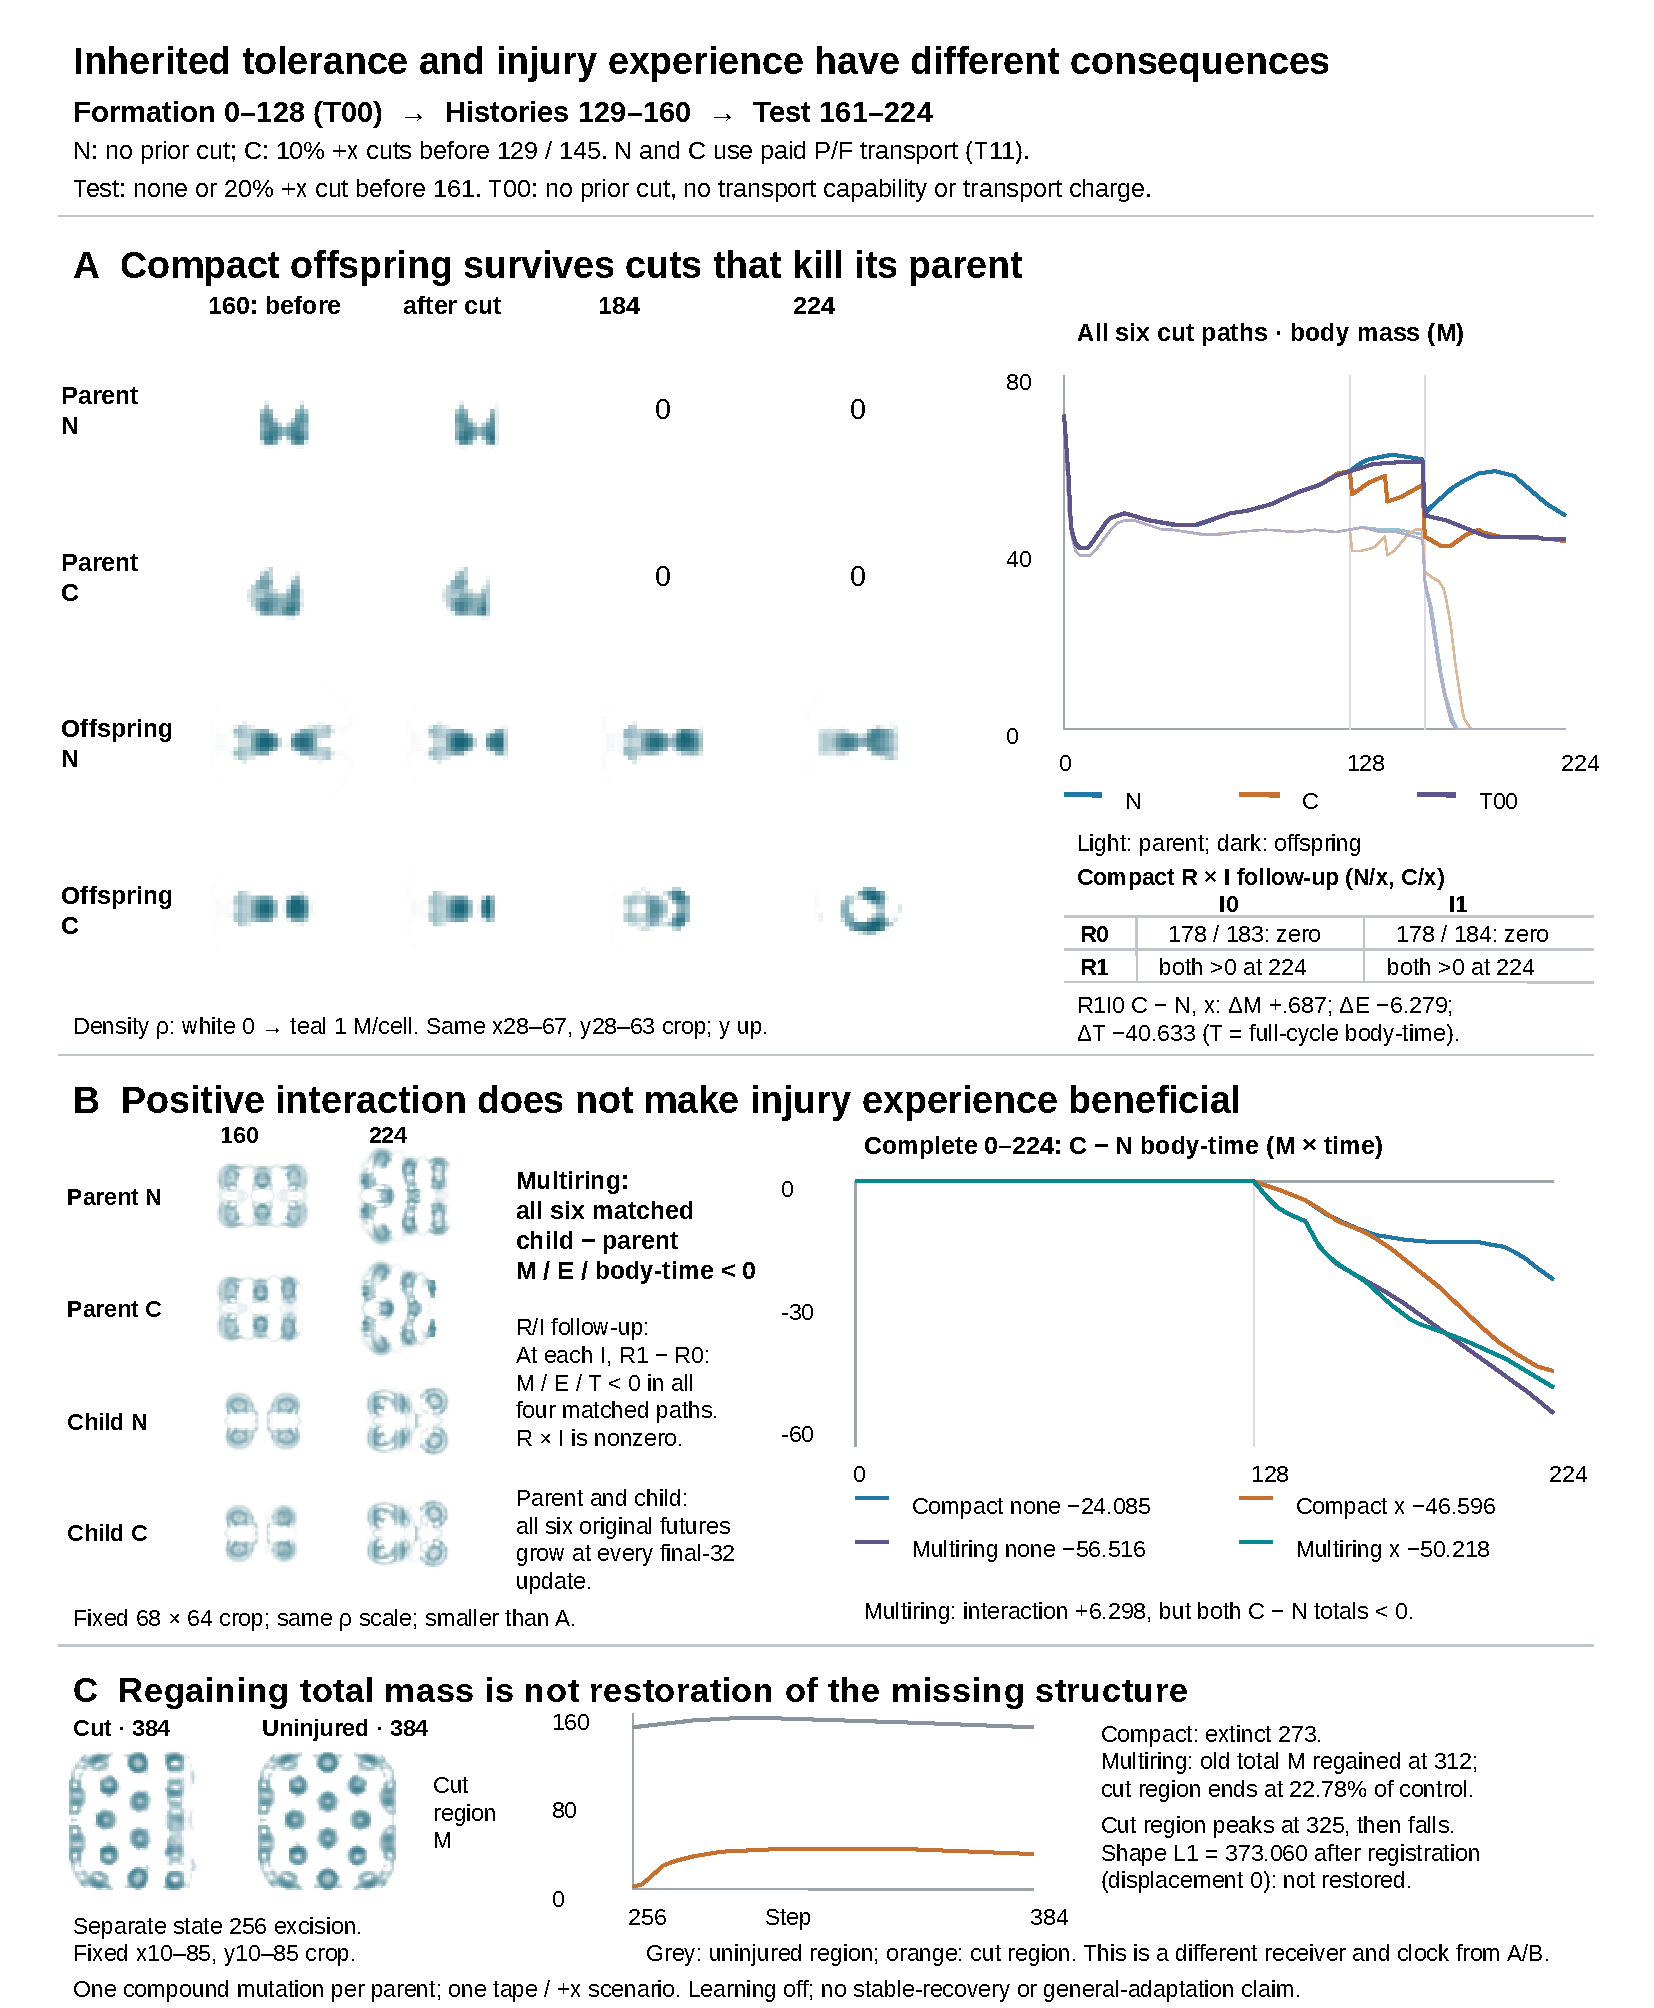
\includegraphics[width=\linewidth,height=.77\textheight,keepaspectratio]{figures/main/inheritance_recovery/regenerative_inheritance_recovery_factorial.pdf}
\caption{\textbf{Inherited tolerance, injury experience and local restoration are distinct.} \textbf{A,} Compact parent/offspring fields and complete challenged paths preserve parental extinction and zero tails. A separate rule--initial matrix shows survival through 224 under both offspring-rule combinations; experienced-minus-naive energy and body-time can nevertheless fall. R contains both kernels and complete response parameters; I contains density, energy, founder and polarity fields. \textbf{B,} The multiring offspring loses in all six matched paths, and the rule cross remains adverse under both I. Both offspring's complete experienced-minus-naive body-time paths are negative. \textbf{C,} An independent state-256 excision receiver regains total mass while its fixed original cut region remains depleted and later shrinks. Original coordinates, terminal uninjured reference and local trajectories distinguish total growth from restoration. Panels have distinct clocks and dependent paths; no learning or general recovery is established.}
\label{fig:inheritance-recovery}\end{figure}
